\noindent En esta sección se busca minimizar el error promedio del primer día para las volatilidades de cada pilar \textit{Delta}, mediante la ecuación \ref{error} planteada anteriormente.\\\\
\noindent Para este caso, se hará uso de los parámetros iniciales previamente estimados para la primera iteración, utilizando el modelo de \textit{Heston} para calcular los precios, para posteriormente, utilizando el algoritmo de \textit{Newton-Raphson}, lograr obtener las volatilidades implícitas de nuestro modelo, para finalmente calcular el valor del error $\epsilon$.\\\\
\noindent Una vez obtenido dicho error, se procedió a iterar el algoritmo utilizando un optimizador, el cual para este caso resultó ser \textit{Fmincon}, disponible en \textit{Matlab}, con tal de encontrar el conjunto de parámetros que minimizan $\epsilon$, y a su vez, entreguen valores coherentes. Cabe destacar que para la minimización del error, se consideraron  las siguientes restricciones:
\begin{equation*}
	0\le \nu	\le1
\end{equation*}
\begin{equation*}
0	\le \Theta	\le100
\end{equation*}
\begin{equation*}
	0\le \omega	\le1
\end{equation*}
\begin{equation*}
0	\le \xi	\le0.5
\end{equation*}
\begin{equation*}
-0.9	\le \rho	\le0.9
\end{equation*}

\noindent Los parámetros obtenidos para el primer día se muestran en la siguiente tabla:

\begin{table}[h]
\begin{center}
\begin{tabular}{| r | l | c |}
\hline 
Parámetros & Valores  \\ \hline
$\nu_1$ & $0.0097^2$  \\
$\Theta$ & 0.6593  \\
$\omega$ & 0.0243    \\
$\xi$ & 0.2869  \\
$\rho$ & -0.0141 \\ \hline
\end{tabular}
\caption{Parámetros $t_1$}
\label{tab:parametros1}
\end{center}
\end{table}

\noindent Por otra parte, el error promedio calculado utilizando la formula \ref{error} es de 0.0096, mientras que el mismo error medido de forma porcentual toma un valor de 9.633\%. Para el cálculo del error en este ultimo caso, se utilizó la siguiente formula:

\begin{equation}
\epsilon_{\%}=\frac{1}{N} \cdot \sum_{i, j}\left|   \frac{\sigma_{i j}^{m o d e l}}{\sigma_{i j}^{m a r k e t}}-1     \right|
\end{equation}

\noindent Finalmente se muestra la curva Smile para los diferentes tenores, utilizando la volatilidad de nuestro modelo como la de mercado, obteniendo las siguientes gráficas:

\begin{figure}[H]
    \begin{center}
    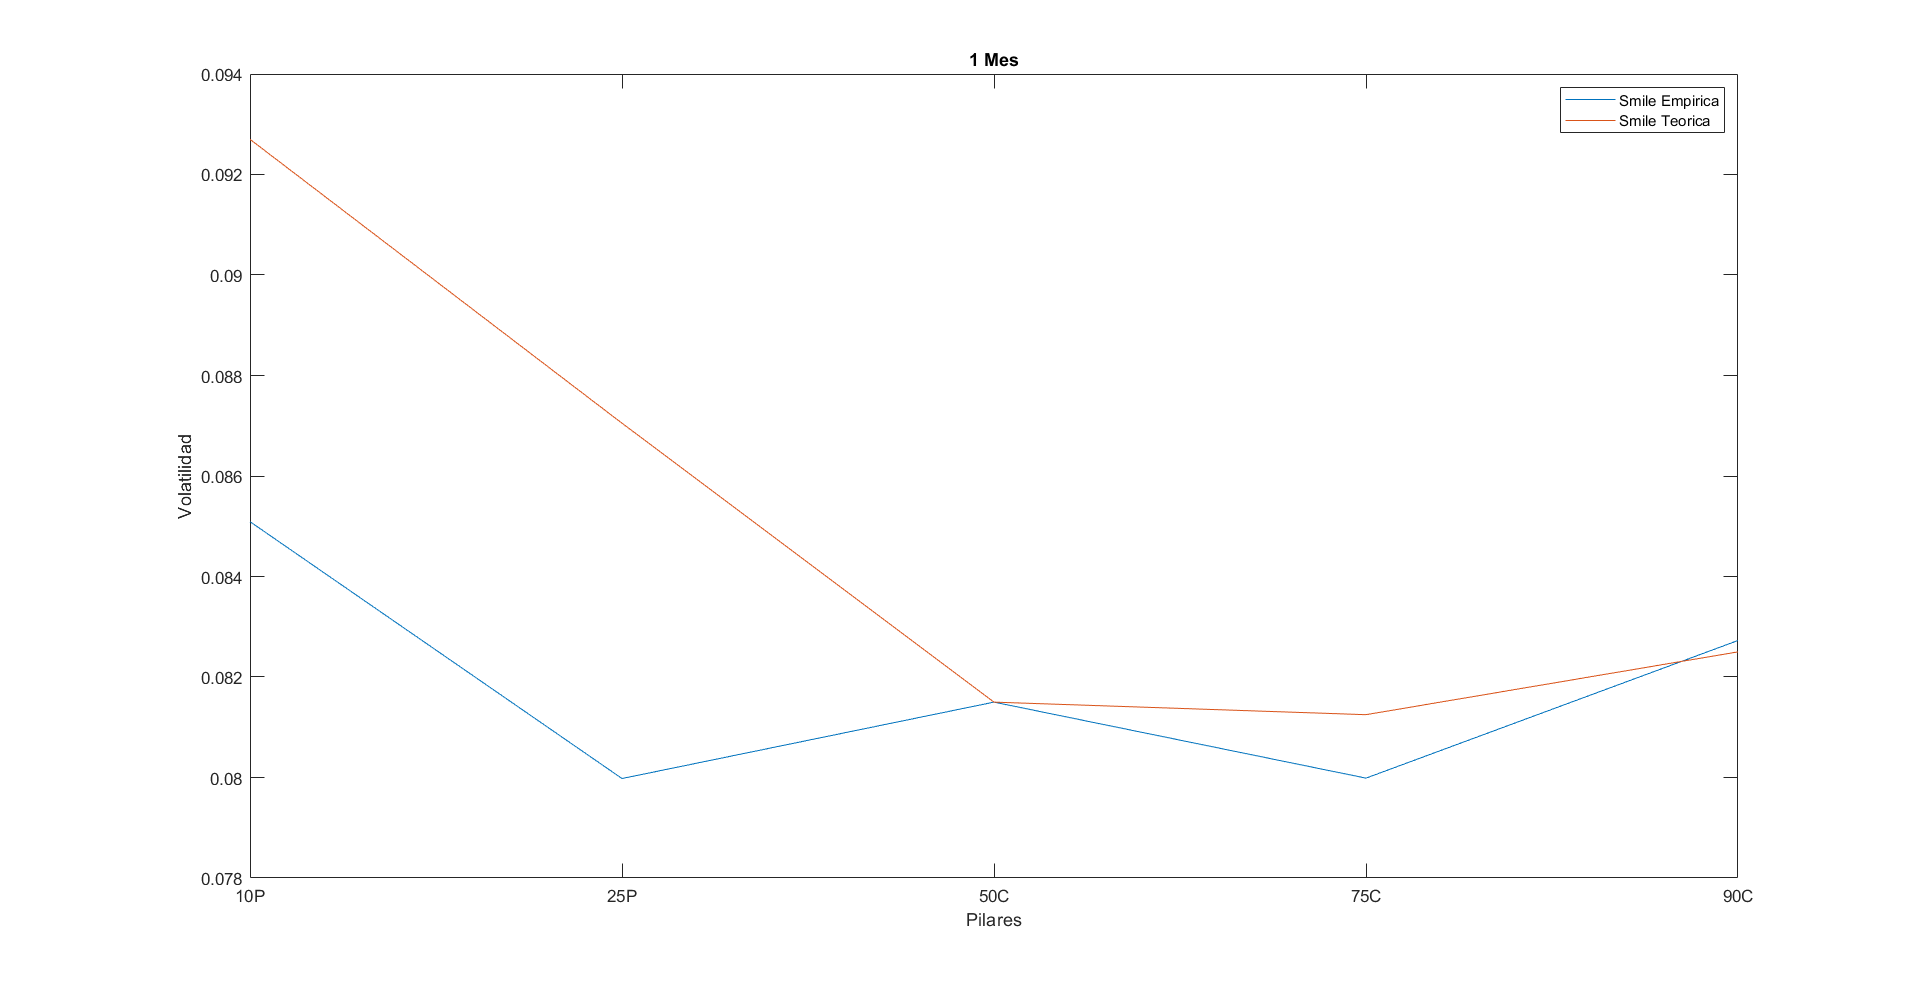
\includegraphics[width = 14cm]{figures/Smile2d1Mes.png}
    \caption{Curva Smile 1 Mes}
    \label{1SmileDia1} %El label permite citar el gráfico, pero es para más adelante
    \end{center}
\end{figure}
\begin{figure}[H]
    \begin{center}
    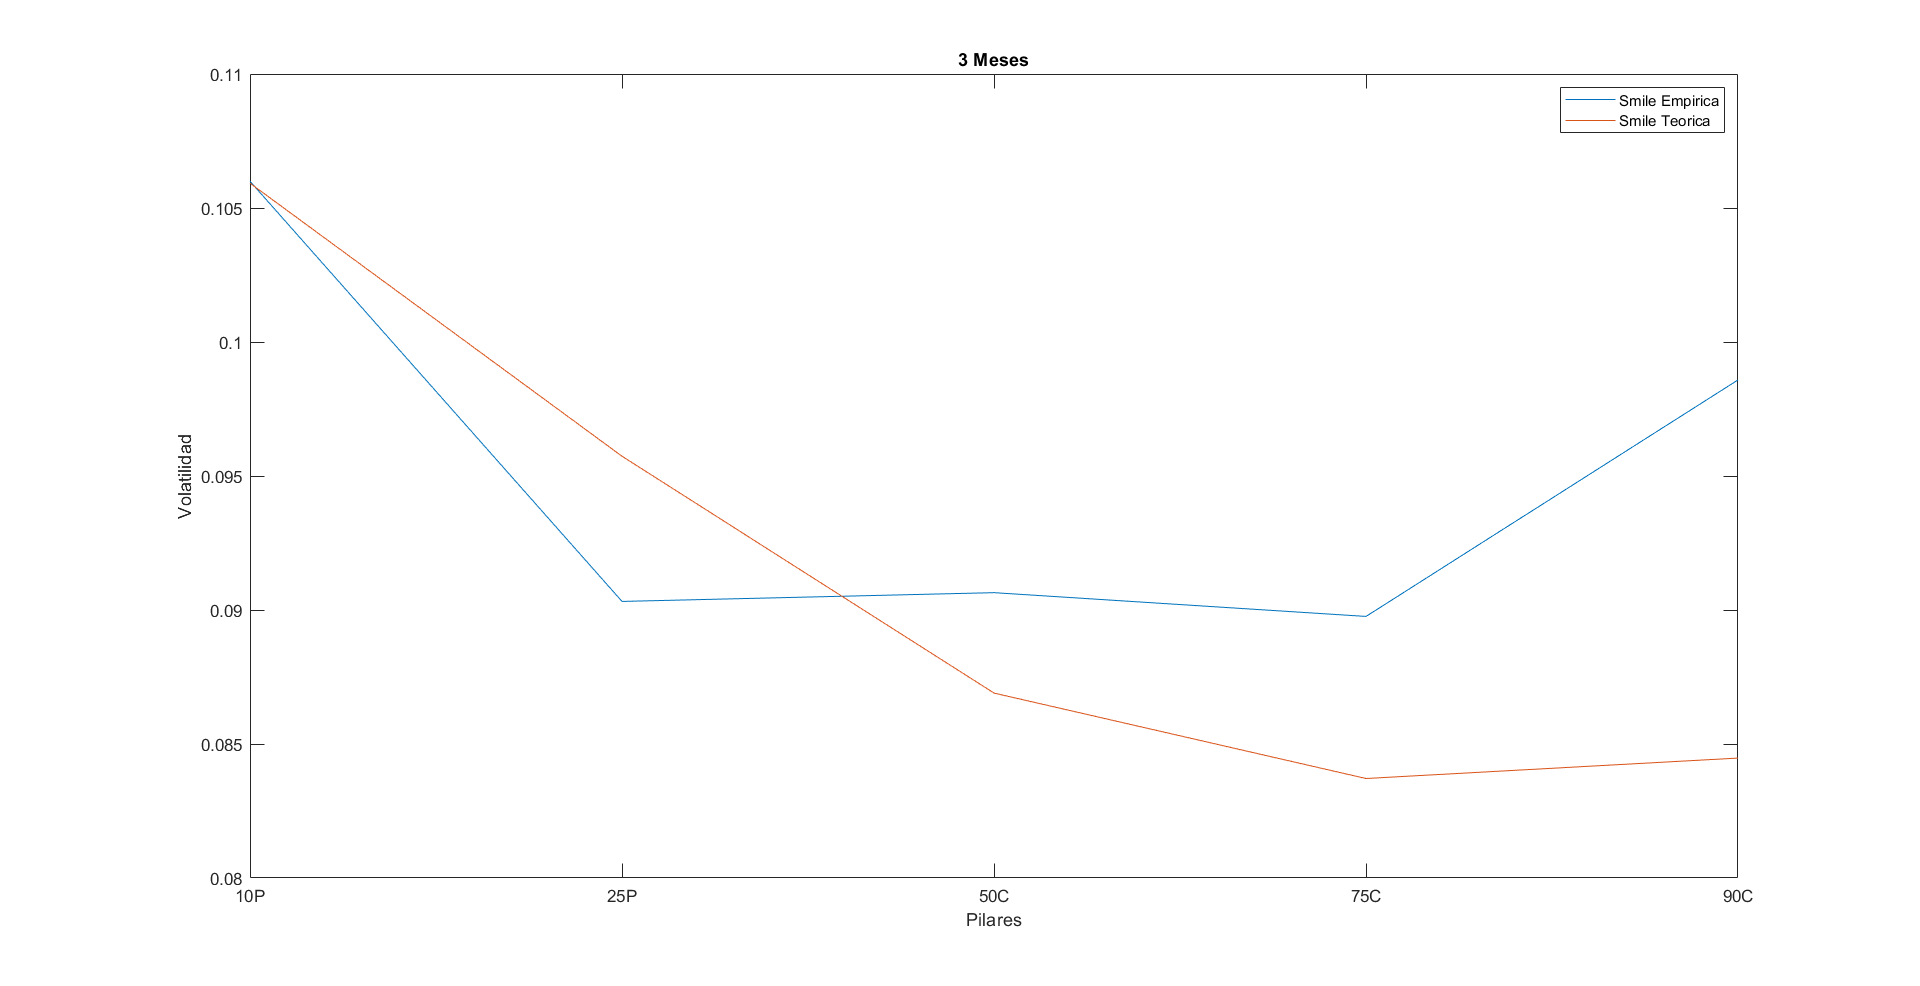
\includegraphics[width = 14cm]{figures/Smile2d3Meses.png}
    \caption{Curva Smile 3 Meses}
    \label{2SmileDia1} %El label permite citar el gráfico, pero es para más adelante
    \end{center}
\end{figure}
\begin{figure}[H]
    \begin{center}
    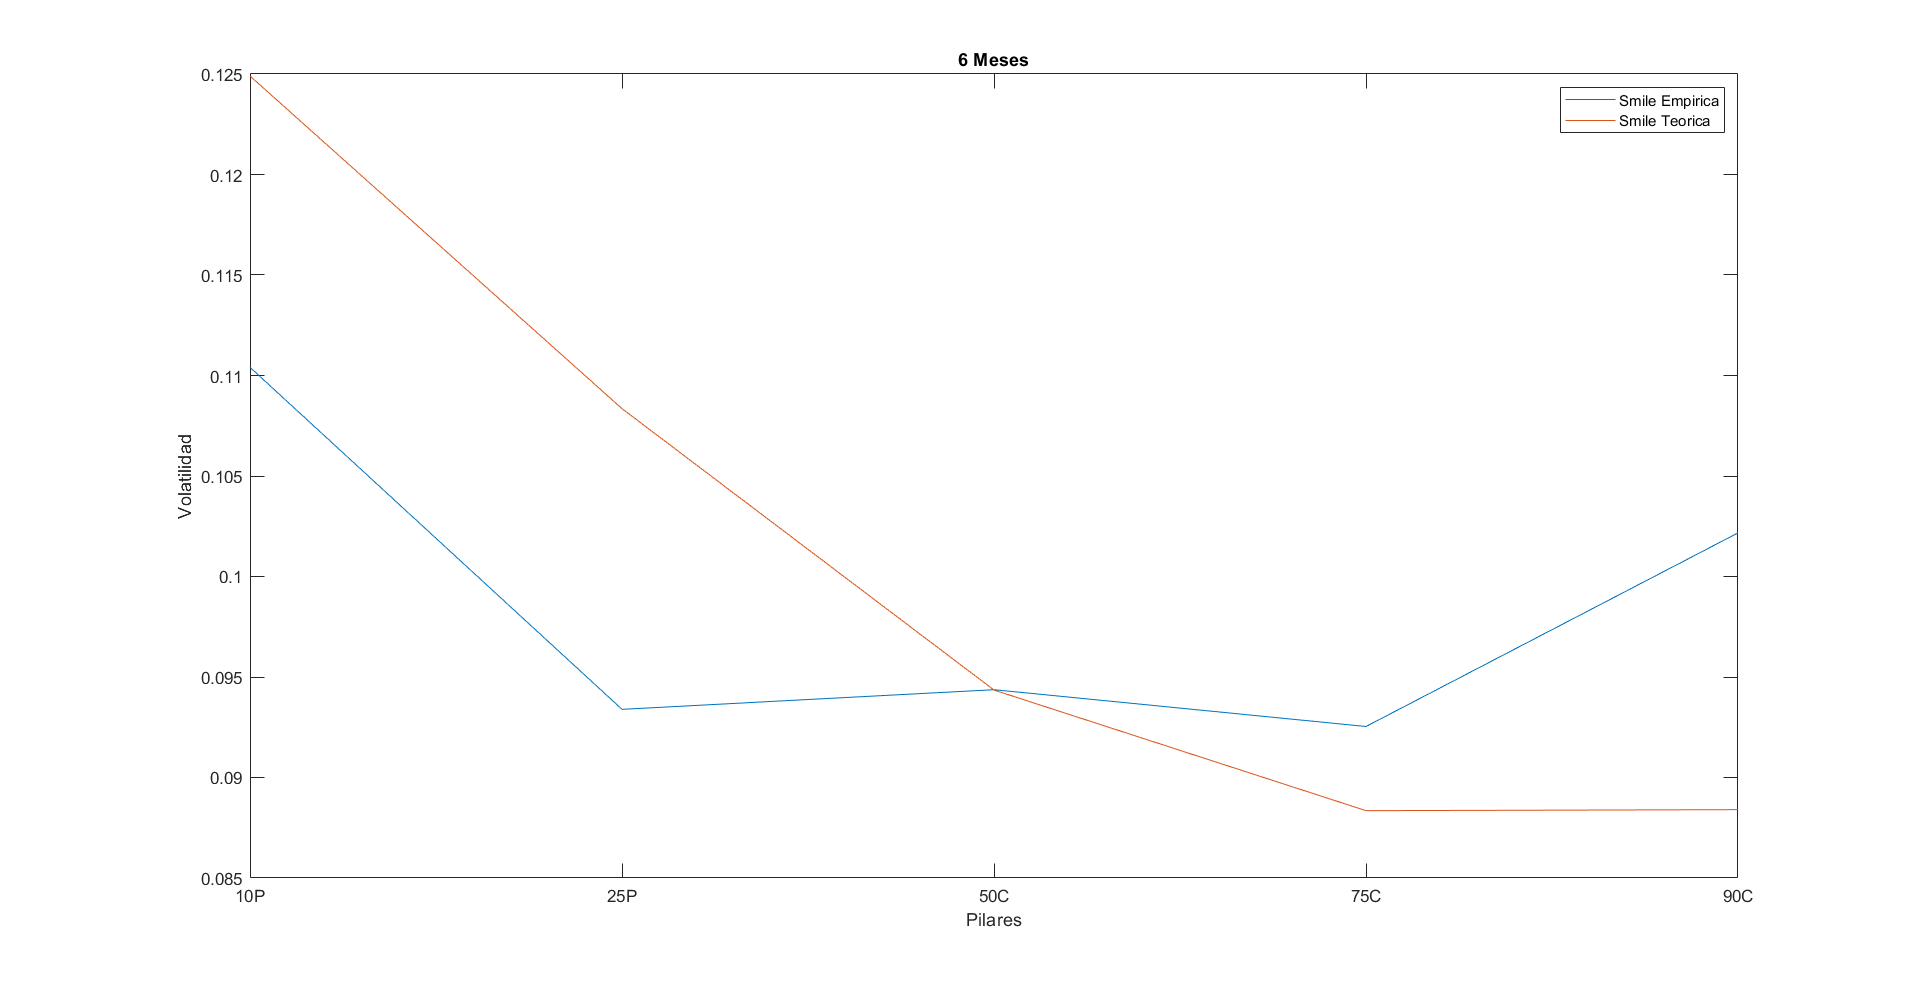
\includegraphics[width = 14cm]{figures/Smile2d6Meses.png}
    \caption{Curva Smile 6 Meses}
    \label{3SmileDia1} %El label permite citar el gráfico, pero es para más adelante
    \end{center}
\end{figure}
\begin{figure}[H]
    \begin{center}
    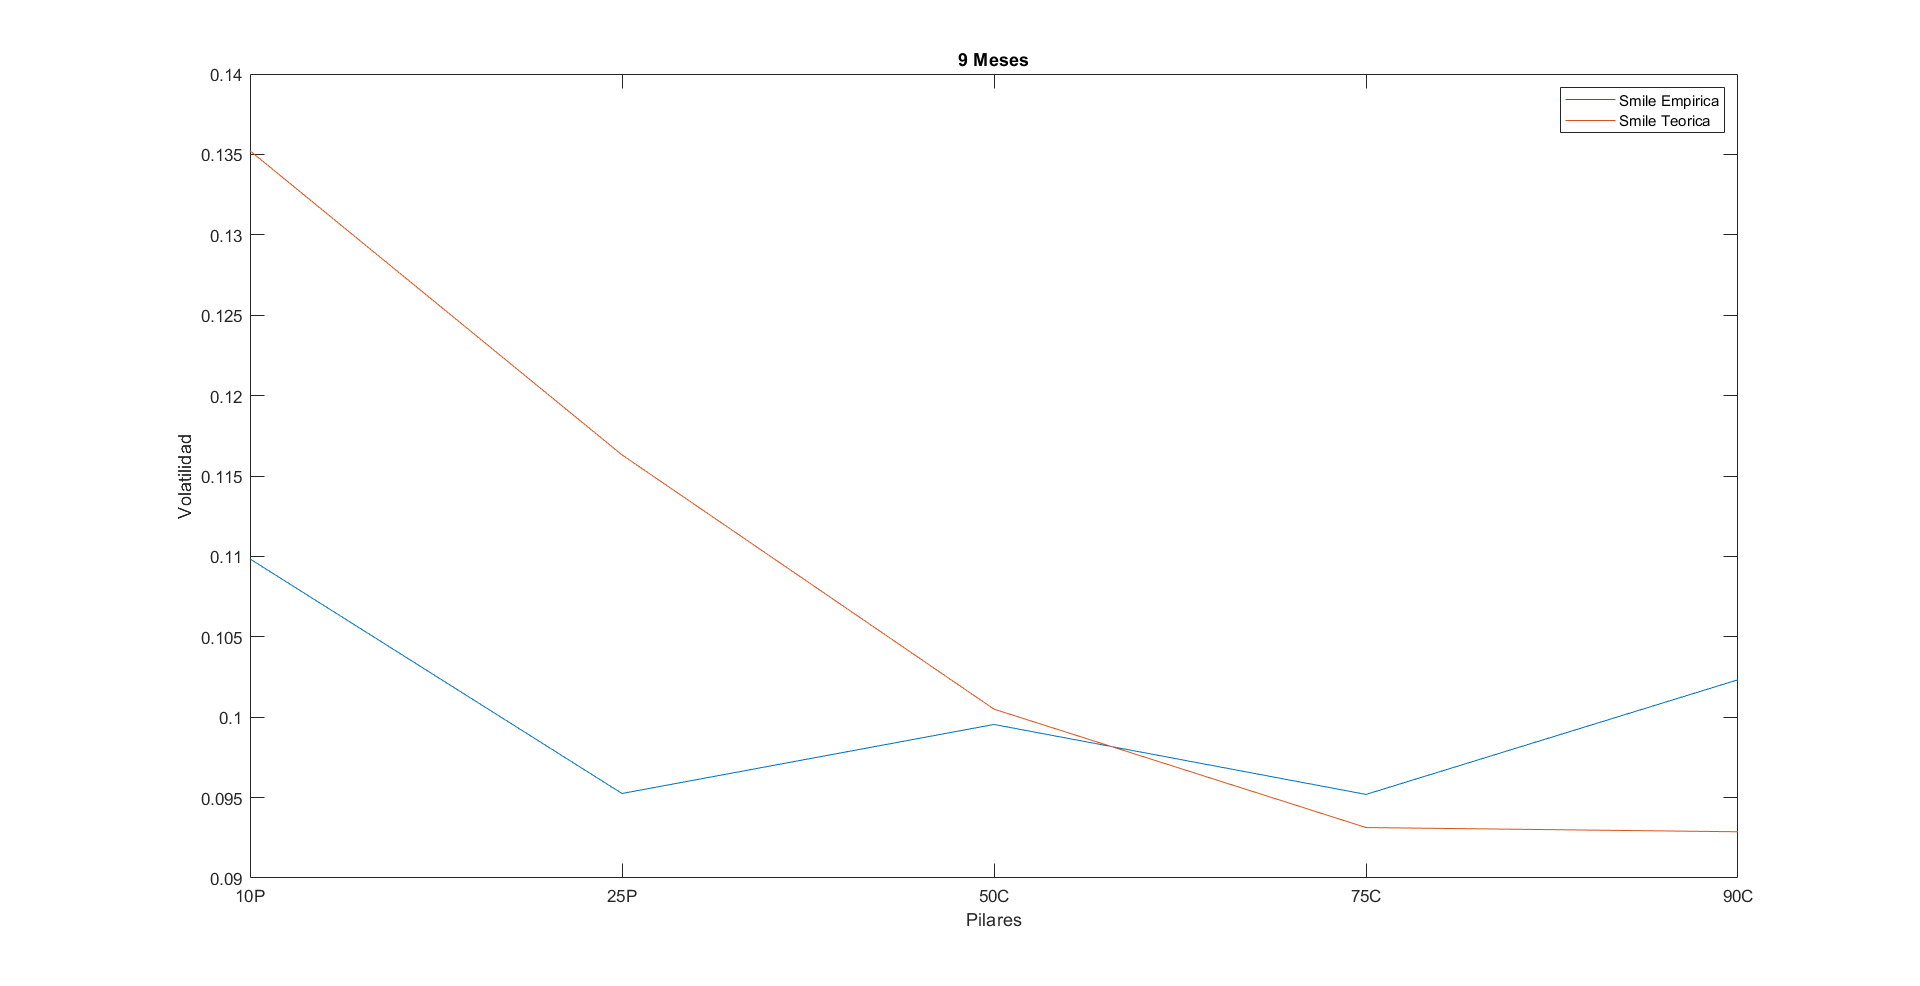
\includegraphics[width = 14cm]{figures/Smile2d9Meses.png}
    \caption{Curva Smile 9 Meses}
    \label{4SmileDia1} %El label permite citar el gráfico, pero es para más adelante
    \end{center}
\end{figure}
\begin{figure}[H]
    \begin{center}
    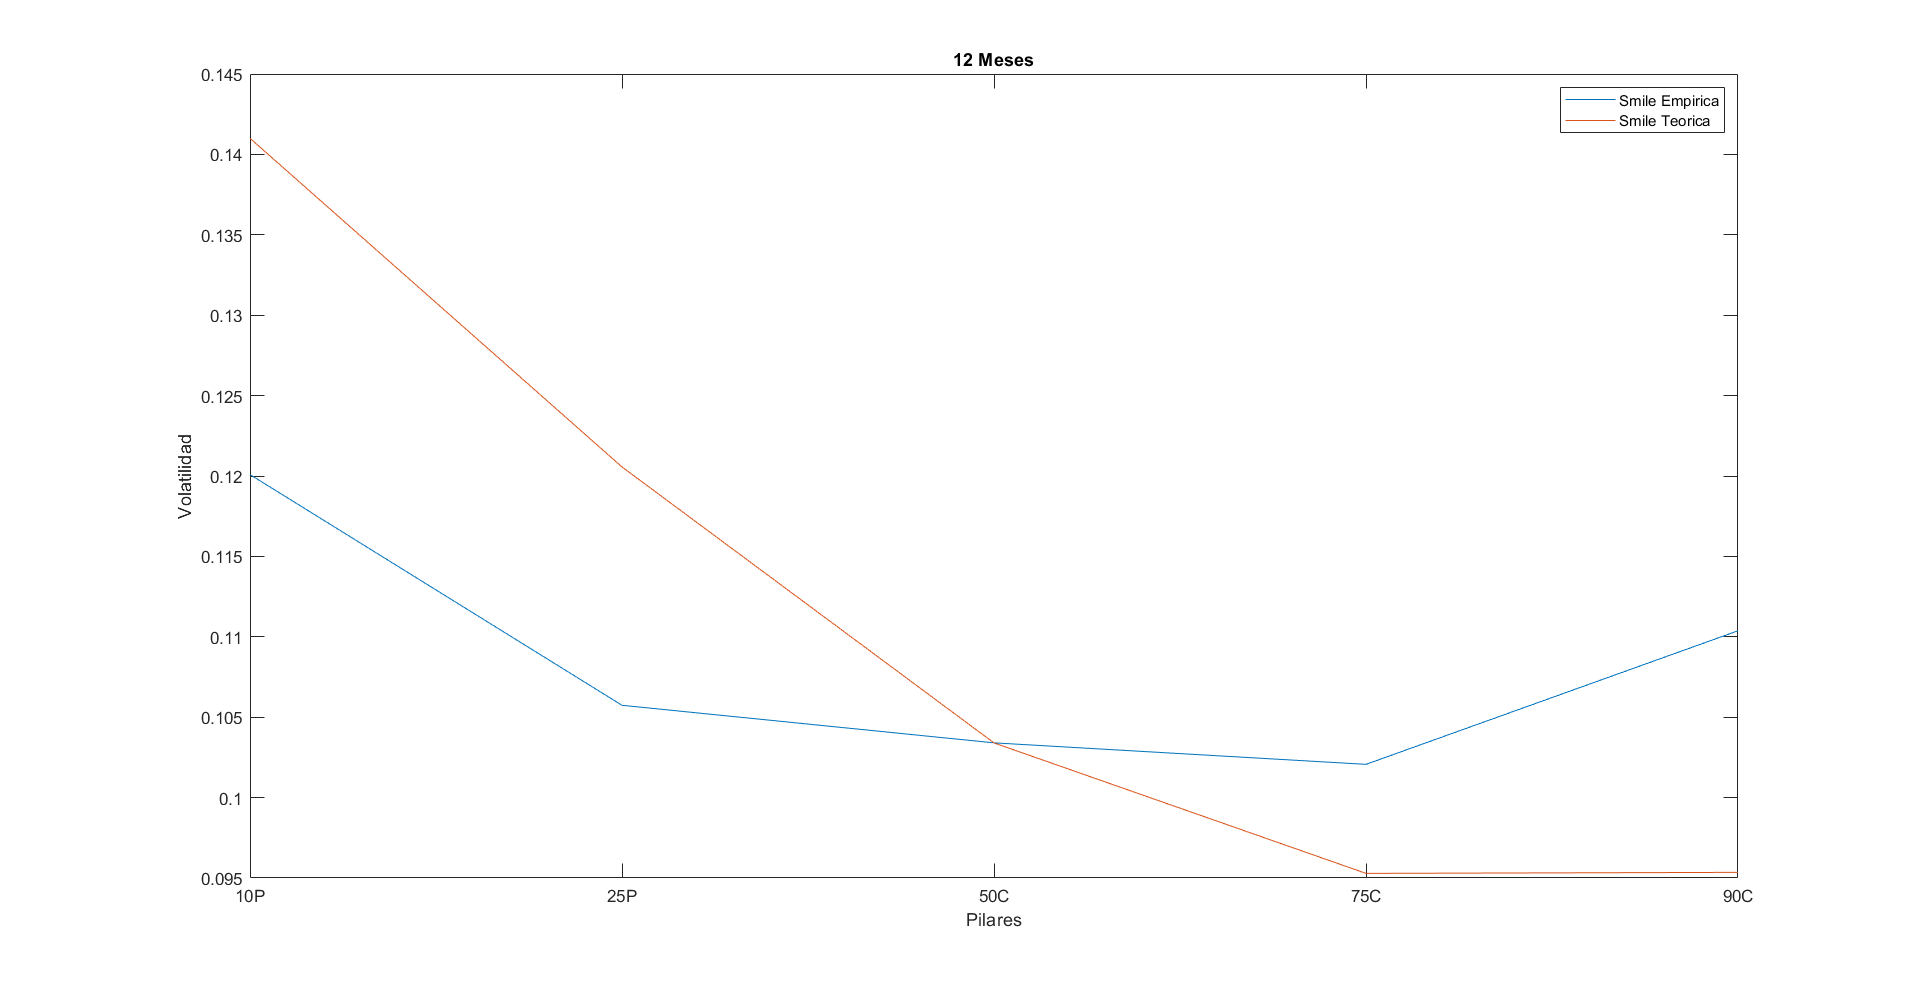
\includegraphics[width = 14cm]{figures/Smile2d12Meses.png}
    \caption{Curva Smile 12 Meses}
    \label{5SmileDia1} %El label permite citar el gráfico, pero es para más adelante
    \end{center}
\end{figure}
\newpage